\newif\ifglobal

%%%%%%%%%%%%%%%%%%%%%%%
%%% Compile to view %%%
%%%%%%%%%%%%%%%%%%%%%%%

%%%%%%%%%%%%%%%%%%%%%%%%%%%%%%%%%%%%%%%%%%%%%%%%%%%
%%% Readme:                                     %%%
%%% https://www.overleaf.com/read/bwdjvfjksvjy/ %%%
%%%%%%%%%%%%%%%%%%%%%%%%%%%%%%%%%%%%%%%%%%%%%%%%%%%

% >>> M?: marks a module setting number or important notice

% >>> M4: Set {./relative-path} to external files for this module <<<
\def \modulefiles {./04-RMT}
% To add an external file, use:
% (Replace '---' with actual filename)
% '\input{\modulefiles/tables/---.tex}' for tables
% '\includegraphics{\modulefiles/figures/---}' for figures
% '\subfile{\modulefiles/---}' for register files


% >>> M1: This module is in global project? <<<
% 'YES' - uncomment; 'NO' - comment out
\globaltrue

\ifglobal
    \documentclass[main\_\_EN.tex]{subfiles}
   
\else
    \documentclass[openany, 10pt]{book}

    % >>> M2: In ./00-shared/preamble-trm-module, also find
    %         settings for visibility of todo notes, watermark <<<
    \usepackage{preamble-trm-module}
    
    \usepackage{ctex}
    % >>> M3: Temporary labels in English,
    %         you can add your own labels there <<<
    \myexternaldocument{./00-shared/temp-labels-en}

\fi %\ifglobal


\setcounter{secnumdepth}{4}


% >>> M5: If this module needs any updates in
% './00-shared/preamble-trm-module.sty'
% (include additional package, etc.), contact your module PM
% or create the file './00-shared/changelog.tex' make the
% necessary updates yourself and document them in this file <<<


\begin{document}


% Sets language into which pre-defined bits of text are translated
\selectlanguage{english}

% Do not delete this block
\ifglobal
% Add the following front matter if
% this module is outside of global project
\else
    \InputIfFileExists{readme}{}{}
    {\let\clearpage\relax \listoftodos}
    \tableofcontents
    %\listoftables
    %\listoffigures
\fi


%%%%%%%%%%%%%%%%%%%%%%%%%
%%% TRM Module Begins %%%
%%%%%%%%%%%%%%%%%%%%%%%%%

\hypertarget{rmt}{}
\chapter{Remote Control Peripheral (RMT)}
\label{mod:rmt}


\section{Overview}
The RMT (Remote Control) module is designed to send and receive infrared remote control signals. A variety of remote control protocols are supported. The RMT module converts pulse codes stored in the module's built-in RAM into output signals, or converts input signals into pulse codes and stores them back in RAM. Optionally, the RMT module modulates its output signals with a carrier wave, or demodulates and filters its input signals.

The RMT module has four channels, numbered from zero to three. Channels 0 \verb+~+ 1 (TX channels) are dedicated to transmit signals, and channels 2 \verb+~+ 3 (RX channels) to receive signals. Each TX/RX channel has the same functionality controlled by a dedicated set of registers and is able to independently either transmit or receive data. TX channels are indicated by \regindex{n} which is used as a placeholder for the channel number, and by \regindex{m} for RX channels.

\section{Features}
\begin{itemize}
\item Two TX channels
\item Two RX channels
\item Support multiple channels (programmable) transmitting data simultaneously
\item Four channels share a 192 x 32-bit RAM
\item Support modulation on TX pulses
\item Support filtering and demodulation on RX pulses
\item Wrap TX mode
\item Wrap RX mode
\item Continuous TX mode
\end{itemize}

\section{Functional Description}
\subsection{RMT Architecture}
\begin{figure}[H]
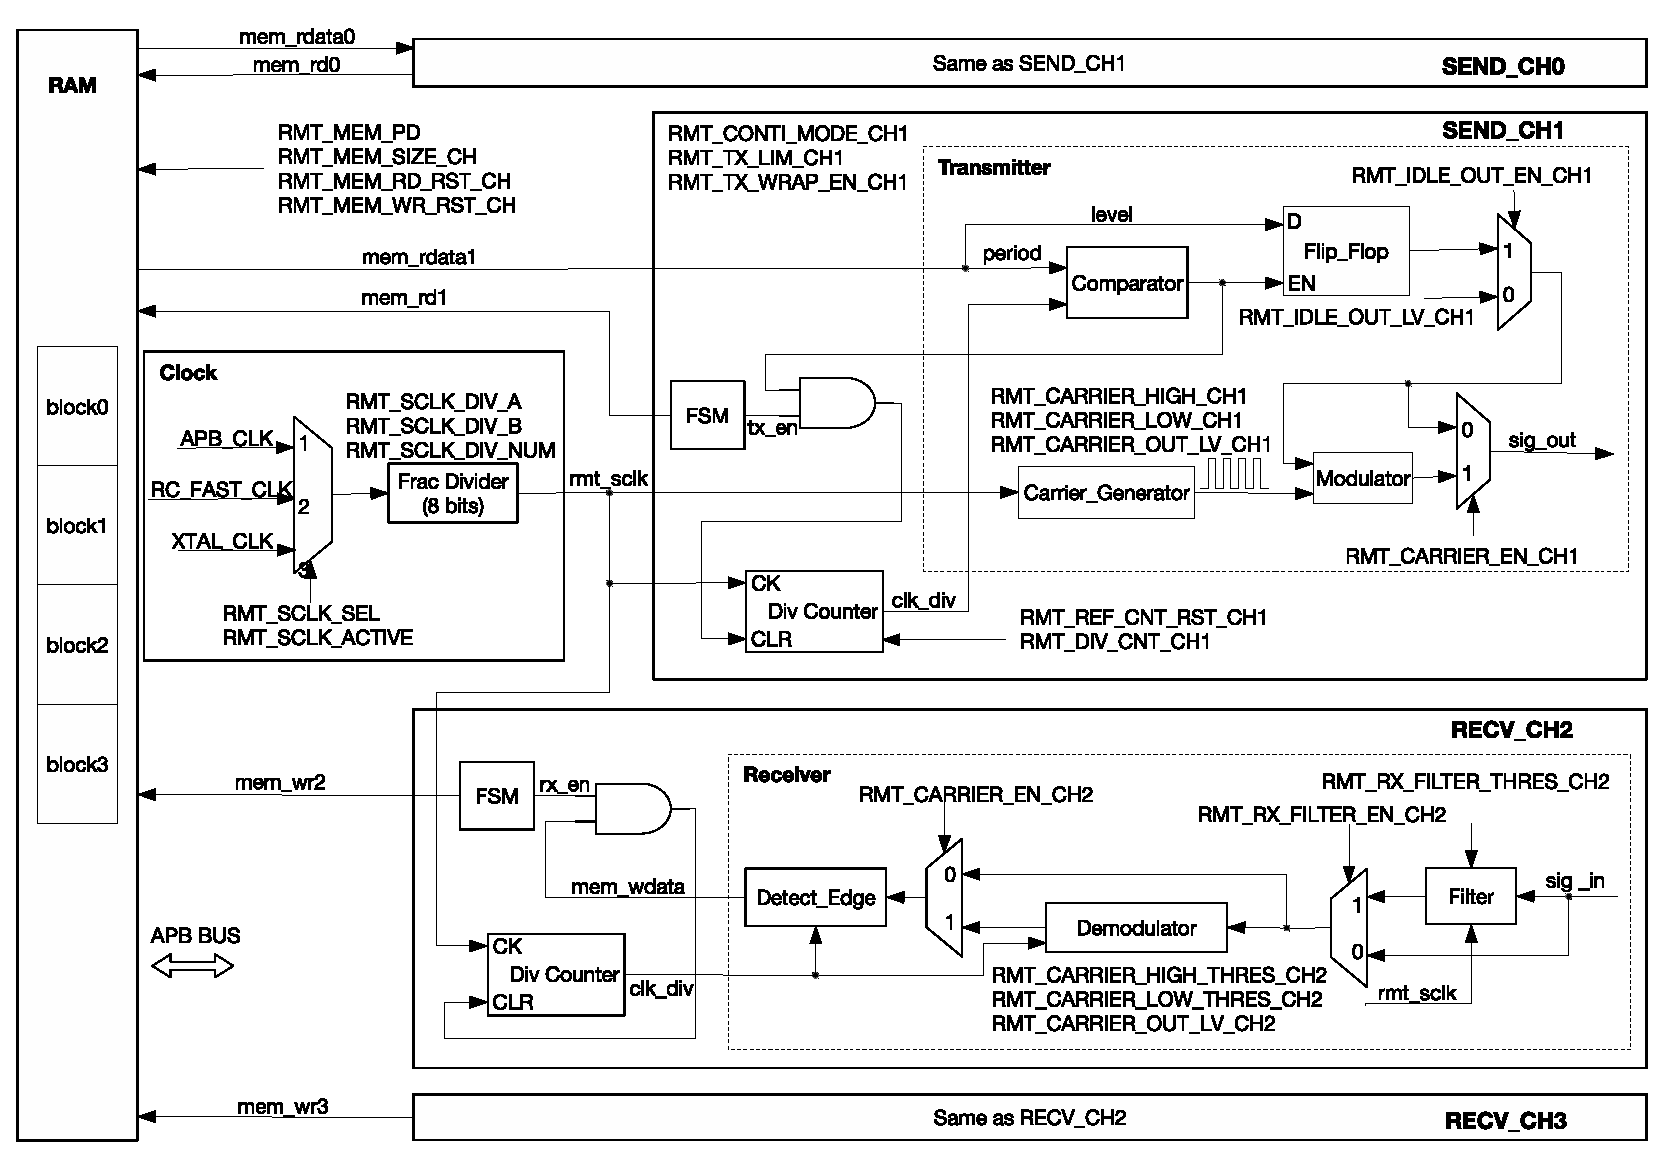
\includegraphics[width=1.0\textwidth]{./04-RMT/figures/rmt_architecture_20221213}
\centering
\caption{RMT Architecture} \label{Figure:RMT2-1}
\end{figure}
The RMT module has four independent channels, two of which are TX channels and the other two are RX channels. Each TX channel has its own clock-divider counter, state machine, and transmitter. Each RX channel also has its own clock-divider counter, state machine, and receiver. The four channels share a 192 x 32-bit RAM.

\subsection{RMT RAM}
\begin{figure}[H]
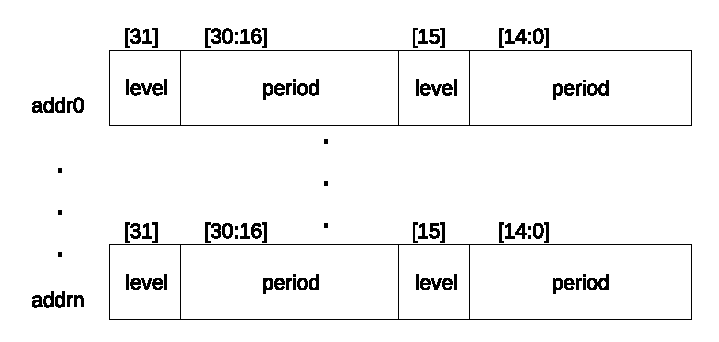
\includegraphics[width=0.5\textwidth]{./04-RMT/figures/rmt_data_structure.eps}
\centering
\caption{Format of Pulse Code in RAM} \label{Figure:RMT2-2}
\end{figure}
Figure \ref{Figure:RMT2-2} shows the format of pulse code in RAM. Each pulse code contains a 16-bit entry with two fields, level and period. 
\begin{itemize}
    \item Level (0 or 1): indicates a low-/high-level value was received or is going to be sent.
    \item Period: points out how many clk\_div clock cycles the level lasts for, see Figure \ref{Figure:RMT2-1}. 
\end{itemize}
A zero (0) period is interpreted as a transmission end-marker. If the period is not an end-marker, its value is limited by APB clock and RMT clock: 

\begin{equation}\label{eq:rmt-period-value}
5 \times T_{apb\_clk} + 6 \times T_{rmt\_sclk} < period \times T_{clk\_div}
\end{equation}

\begin{tiplisting}
RMT clock and APB clock must satisfy the following relation:
    \begin{equation}
    1.5 \times T_{apb\_clk} < 9 \times T_{rmt\_sclk}
    \end{equation}
\end{tiplisting}

The RAM is divided into four 48 x 32-bit blocks. By default, each channel uses one block, block zero for channel zero, block one for channel one, and so on. 

If the data size of one single transfer is larger than this block size of TX channel \regindex{n} or RX channel \regindex{m}, users can configure the channel 
\begin{itemize}
    \item to enable wrap mode by setting RMT\_MEM\_TX\_WRAP\_EN\_CH\regindex{n}/\regindex{m}.
    \item or to use more blocks by configuring RMT\_MEM\_SIZE\_CH\regindex{n}/\regindex{m}.
\end{itemize}
Setting RMT\_MEM\_SIZE\_CH\regindex{n}/\regindex{m} > 1 allows channel \regindex{n}/\regindex{m} to use the memory of subsequent channels, block (\regindex{n}/\regindex{m}) \verb+~+ block (\regindex{n}/\regindex{m} + RMT\_MEM\_SIZE\_CH\regindex{n}/\regindex{m} -1). If so, the subsequent channels  \regindex{n}/\regindex{m} + 1 \verb+~+ \regindex{n}/\regindex{m} + RMT\_MEM\_SIZE\_CH\regindex{n}/\regindex{m} - 1 can not be used once their RAM blocks are occupied. 

Note that the RAM used by each channel is mapped from low address to high address. In such mode, channel 0 is able to use the RAM blocks for channels 1, 2 and 3 by setting RMT\_MEM\_SIZE\_CH0, but channel 3 can not use the blocks for channels 0, 1, or 2. Therefore, the maximum value of RMT\_MEM\_SIZE\_CH\regindex{n} should not exceed (4 - \regindex{n}) and the maximum value of RMT\_MEM\_SIZE\_CH\regindex{m} should not exceed (2 - \regindex{m}).

The RMT RAM can be accessed via APB bus, or read by the transmitter and written by the receiver. To avoid any possible access conflict between the receiver and the APB bus, RMT can be configured to designate the RAM block's owner, be it the receiver or the APB bus, by configuring RMT\_MEM\_OWNER\_CH\regindex{m}. If this ownership is violated, a flag signal RMT\_CH\regindex{m}\_OWNER\_ERR will be generated. 

APB bus is able to access RAM in FIFO mode and in Direct Address (NONFIFO) mode, depending on the configuration of RMT\_FIFO\_MASK:
\begin{itemize}
    \item 1: use NONFIFO mode;
    \item 0: use FIFO mode. 
\end{itemize}

In FIFO mode, the APB reads data from or writes data to RAM via a fixed address stored in \hyperref[regdesc:RMTCHNDATAREG]{RMT\_CH\regindex{n}/\regindex{m}DATA\_REG}.

In NONFIFO mode, the APB writes data to or reads data from a continuous address range. The write-starting address of TX channel \regindex{n} is: RMT base address + 0x400 + \regindex{n}x48. The access address for the second data and the following data are RMT base address + 0x400 + \regindex{n}x48 + 0x4, and so on, incremented by 0x4. The read-starting address of RX channel \regindex{m} is: RMT base address + 0x460 + \regindex{m}x48. The access address for the second data and the following data are RMT base address + 0x460 + \regindex{m}x48 + 0x4, and so on, incremented by 0x4.

When the RMT module is inactive, the RAM can be put into low-power mode by setting  \hyperref[fielddesc:RMTMEMFORCEPD]{RMT\_MEM\_FORCE\_PD}.

\subsection{Clock}\label{clock}
The clock source of RMT can be APB\_CLK, RC\_FAST\_CLK or XTAL\_CLK, depending on the configuration of RMT\_SCLK\_SEL. RMT clock can be enabled by setting RMT\_SCLK\_ACTIVE. RMT working clock (rmt\_sclk) is obtained by dividing the selected clock source with a fractional divider, see Figure \ref{Figure:RMT2-1}. The divider is: 

$$
RMT\_SCLK\_DIV\_NUM + 1 + RMT\_SCLK\_DIV\_A/RMT\_SCLK\_DIV\_B
$$

For more information, please check Chapter \ref{mod:resclk} \textit{\nameref{mod:resclk}}.

RMT\_DIV\_CNT\_CH\regindex{n}/\regindex{m} is used to configure the divider coefficient of internal clock divider for RMT channels. The coefficient is normally equal to the value of RMT\_DIV\_CNT\_CH\regindex{n}/\regindex{m}, except value 0 that represents coefficient 256. The clock divider can be reset by clearing RMT\_REF\_CNT\_RST\_CH\regindex{n}/\regindex{m}. The clock generated from the divider can be used by the counter (see Figure \ref{Figure:RMT2-1}).

\subsection{Transmitter}

\subsubsection{Normal TX Mode}

When \hyperref[fielddesc:RMTTXSTARTCHN]{RMT\_TX\_START\_CH\regindex{n}} is set, the transmitter of channel \regindex{n} starts reading and sending pulse codes from the starting address of its RAM block. The codes are sent starting from low-address entry. 

When an end-marker (a zero period) is encountered, the transmitter stops the transmission, returns to idle state and generates an  \hyperref[int:RMTCHnTXENDINT]{RMT\_CH\regindex{n}\_TX\_END\_INT} interrupt. Setting \hyperref[fielddesc:RMTTXSTOPCHN]{RMT\_TX\_STOP\_CH\regindex{n}} to 1 also stops the transmission and immediately sets the transmitter back to idle. 

The output level of a transmitter in idle state is determined by the ``level" field of the end-marker or by the content of  \hyperref[fielddesc:RMTIDLEOUTLVCHN]{RMT\_IDLE\_OUT\_LV\_CH\regindex{n}}, depending on the configuration of  \hyperref[fielddesc:RMTIDLEOUTENCHN]{RMT\_IDLE\_OUT\_EN\_CH\regindex{n}}. 

To implement the above-mentioned configurations, please set RMT\_CONF\_UPDATE\_CH\regindex{n} first. For more information, see Section \ref{conf_update}.


\subsubsection{Wrap TX Mode}

To transmit more pulse codes than can be fitted in the channel's RAM, users can enable wrap TX mode by setting \hyperref[fielddesc:RMTMEMTXWRAPENCHN]{RMT\_MEM\_TX\_WRAP\_EN\_CH\regindex{n}}. In this mode, the transmitter sends the data from RAM in loops till an end-marker is encountered.

For example, if  \hyperref[fielddesc:RMTMEMSIZECHN]{RMT\_MEM\_SIZE\_CH\regindex{n}} = 1, the transmitter starts sending data from the address 48 * \regindex{n}, and then the data from higher RAM address. Once the transmitter finishes sending the data from (48 * (\regindex{n} + 1) - 1), it continues sending data from 48 * \regindex{n} again till an end-marker is encountered. Wrap mode is also applicable for \hyperref[fielddesc:RMTMEMSIZECHN]{RMT\_MEM\_SIZE\_CH\regindex{n}} > 1.

When the size of transmitted pulse codes is larger than or equal to the value set by  \hyperref[fielddesc:RMTTXLIMCHN]{RMT\_TX\_LIM\_CH\regindex{n}}, an \hyperref[int:RMTCHnTXTHREVENTINT]{RMT\_CH\regindex{n}\_TX\_THR\_EVENT\_INT} interrupt is triggered. In wrap mode,  \hyperref[fielddesc:RMTTXLIMCHN]{RMT\_TX\_LIM\_CH\regindex{n}} can be set to a half or a fraction of the size of the channel's RAM block. When an  \hyperref[int:RMTCHnTXTHREVENTINT]{RMT\_CH\regindex{n}\_TX\_THR\_EVENT\_INT} interrupt is detected by software, the already used RAM region can be updated with new pulse codes. In this way the transmitter can seamlessly send unlimited pulse codes in wrap mode.

To update the configuration of RMT\_MEM\_TX\_WRAP\_EN\_CH\regindex{n}, RMT\_MEM\_SIZE\_CH\regindex{n}, and RMT\_TX\_LIM\_CH\regindex{n}, please set RMT\_CONF\_UPDATE\_CH\regindex{n} first. For more information, see Section \ref{conf_update}.

\subsubsection{TX Modulation}

Transmitter output can be modulated with a carrier wave by setting  \hyperref[fielddesc:RMTCARRIERENCHN]{RMT\_CARRIER\_EN\_CH\regindex{n}}. The carrier waveform is configurable. 

In a carrier cycle, high level lasts for (\hyperref[fielddesc:RMTCARRIERHIGHCHN]{RMT\_CARRIER\_HIGH\_CH\regindex{n}} + 1) rmt\_sclk cycles, while low level lasts for (\hyperref[fielddesc:RMTCARRIERLOWCHN]{RMT\_CARRIER\_LOW\_CH\regindex{n}} + 1) rmt\_sclk cycles. When  \hyperref[fielddesc:RMTCARRIEROUTLVCHN]{RMT\_CARRIER\_OUT\_LV\_CH\regindex{n}} is set, carrier wave is added on the high-level of output signals; while  \hyperref[fielddesc:RMTCARRIEROUTLVCHN]{RMT\_CARRIER\_OUT\_LV\_CH\regindex{n}} is cleared, carrier wave is added on the low-level of output signals. 

Carrier wave can be added on all output signals during modulation, or just added on valid pulse codes (the data stored in RAM), depending on the configuration of \hyperref[fielddesc:RMTCARRIEREFFENCHN]{RMT\_CARRIER\_EFF\_EN\_CH\regindex{n}}: 
\begin{itemize}
    \item 0: add carrier wave on all output signals;
    \item 1: add carrier wave only on valid signals.
\end{itemize}

To implement the modulation configuration, please set RMT\_CONF\_UPDATE\_CH\regindex{n} first. For more information, see Section \ref{conf_update}.

\subsubsection{Continuous TX Mode}

This continuous TX mode can be enabled by setting RMT\_TX\_CONTI\_MODE\_CH\regindex{n}. In this mode, the transmitter sends the pulse codes from RAM in loops. 
\begin{itemize}
    \item If an end-marker is encountered, the transmitter starts transmitting the first data again. 
    \item If no end-marker is encountered, the transmitter starts transmitting the first data again after the last data is transmitted.
\end{itemize}

If RMT\_TX\_LOOP\_CNT\_EN\_CH\regindex{n} is set, the loop counting is incremented by 1 each time an end-marker is encountered. If the counting reaches the value set in RMT\_TX \_LOOP\_NUM\_CH\regindex{n}, an RMT\_CH\regindex{n}\_TX\_LOOP\_INT is generated. 

In an end-marker, if its period[14:0] is 0, then the period of the previous data must satisfy the following requirement:

\begin{equation}
10 \times T_{apb\_clk} + 19 \times T_{rmt\_sclk} < period \times T_{clk\_div}
\end{equation}

The period of the other data only need to satisfy \hyperref[eq:rmt-period-value]{non-zero period relation}.

To implement the above-mentioned configuration, please set RMT\_CONF\_UPDATE\_CH\regindex{n} first. For more information, see Section \ref{conf_update}.

\subsubsection{Simultaneous TX Mode}

RMT module supports multiple channels transmitting data simultaneously. To use this function, follow the steps below.

\begin{enumerate}
    \item Configure RMT\_TX\_SIM\_CH\regindex{n} to choose which multiple channels are used to transmit data simultaneously.
    \item Set RMT\_TX\_SIM\_EN to enable this transmission mode.
    \item Set RMT\_TX\_START\_CH\regindex{n} for each selected channel, to start data transmitting.
\end{enumerate}

Once the last channel is configured, these channels start transmitting data simultaneously. Due to hardware limitations, there is no guarantee that two channels can start sending data exactly at the same time. The interval between two channels starting transmitting data is within 3 x T$_{clk\_div}$.

To configure RMT\_TX\_SIM\_EN, please set RMT\_CONF\_UPDATE\_CH\regindex{n} first. For more information, see Section \ref{conf_update}.



\subsection{Receiver}

\subsubsection{Normal RX Mode}

The receiver of channel \regindex{m} is controlled by RMT\_RX\_EN\_CH\regindex{m}:
\begin{itemize}
    \item RMT\_RX\_EN\_CH\regindex{m} = 1, the receiver starts working.
    \item RMT\_RX\_EN\_CH\regindex{m} = 0, the receiver stops receiving data.
\end{itemize}

When the receiver becomes active, it starts counting from the first edge of the signal, detecting signal levels and counting clock cycles the level lasts for. Each cycle count is then written back to RAM. 

When the receiver detects no change in a signal level for a number of clock cycles more than the value set by RMT\_IDLE\_THRES\_CH\regindex{m}, the receiver will stop receiving data, return to idle state, and generate an RMT\_CH\regindex{m}\_RX\_END\_INT interrupt.

Please note that RMT\_IDLE\_THRES\_CH\regindex{m} should be configured to a maximum value according to your application, otherwise a valid received level may be mistaken as a level in idle state.

If RAM block of this RX channel is used up by the received data, the receiver will stop receiving data, and generate an  \hyperref[int:RMTCHnERRINT]{RMT\_CH\regindex{m}\_ERR\_INT} interrupt triggered by RAM FULL event.

To implement configuration above, please set RMT\_CONF\_UPDATE\_CH\regindex{m} first. For more information, see Section \ref{conf_update}.

\subsubsection{Wrap RX Mode}

To receive more pulse codes than can be fitted in the channel's RAM, users can enable wrap RX mode for channel \regindex{m} by configuring RMT\_MEM\_RX\_WRAP\_EN\_CH\regindex{m}. In wrap mode, the receiver stores the received data to RAM block of this channel in loops. 

Receiving ends, when the receiver detects no change in a signal level for a number of clock cycles more than the value set by RMT\_IDLE\_THRES\_CH\regindex{m}. The receiver then returns to idle state and generates an RMT\_CH\regindex{m}\_RX\_END\_INT interrupt. 

For example, if RMT\_MEM\_SIZE\_CH\regindex{m} is set to 1, the receiver starts receiving data and stores the data to address 48 * \regindex{m}, and then to higher RAM address. When the receiver finishes storing the received data to address (48 * (\regindex{m} + 1) - 1), the receiver continues receiving data and storing data to the address 48 * \regindex{m} again, till no change is detected on a signal level for more than RMT\_IDLE\_THRES\_CH\regindex{m} clock cycles. Wrap mode is also applicable for RMT\_MEM\_SIZE\_CH\regindex{m} > 1.

An RMT\_CH\regindex{m}\_RX\_THR\_EVENT\_INT is generated when the size of received pulse codes is larger than or equal to the value set by RMT\_RX\_LIM\_CH\regindex{m}. In wrap mode, RMT\_RX\_LIM\_CH\regindex{M}
can be set to a half or a fraction of the size of the channel's RAM block. When an RMT\_CH\regindex{m}\_RX\_THR\_EVENT\_INT interrupt is detected by software, the system will be notified to copy out data stored in already used RMT RAM region, and then the region can be updated by subsequent data. In this way an arbitrary amount of data can be seamlessly received.

To implement the configuration above, please set RMT\_CONF\_UPDATE\_CH\regindex{m} first. For more information, see Section \ref{conf_update}.

\subsubsection{RX Filtering}

Users can enable the receiver to filter input signals by setting RMT\_RX\_FILTER\_EN\_CH\regindex{m} for each channel. The filter samples input signals continuously, and detects the signals which remain unchanged for a continuous RMT\_RX\_FILTER\_THRES\_CH\regindex{m} rmt\_sclk cycles as valid, otherwise, the signals are rejected. Only the valid signals can pass through this filter. The filter removes pulses with a length of less than RMT\_RX\_FILTER\_THRES\_CH\regindex{n} rmt\_sclk cycles.

To implement the configuration above, please set RMT\_CONF\_UPDATE\_CH\regindex{m} first. For more information, see Section \ref{conf_update}.

\subsubsection{RX Demodulation}

Users can enable demodulation function on input signals or on filtered output signals by setting RMT\_CARRIER\_EN\_CH\regindex{m}. RX demodulation can be applied to high-level carrier wave or low-level carrier wave, depending on the configuration of RMT\_CARRIER\_OUT\_LV\_CH\regindex{m}: 
\begin{itemize}
    \item 1: demodulate high-level carrier wave
    \item 0: demodulate low-level carrier wave
\end{itemize}

 Users can configure RMT\_CARRIER\_HIGH\_THRES\_CH\regindex{m} and RMT\_CARRIER\_LOW\_THRES\_CH\regindex{m} to set the thresholds to demodulate high-level carrier wave or low-level carrier wave.
 
 If the high-level of a signal lasts for less than RMT\_CARRIER\_HIGH\_THRES\_CH\regindex{m} clk\_div cycles, or the low-level lasts for less than RMT\_CARRIER\_LOW\_THRES\_CH\regindex{m} clk\_div cycles, such level is detected as a carrier wave and then is filtered out.

To implement the configuration above, please set RMT\_CONF\_UPDATE\_CH\regindex{m} first. For more information, see Section \ref{conf_update}.

\subsection{Configuration Update}\label{conf_update}

To update RMT registers configuration, please set RMT\_CONF\_UPDATE\_CH\regindex{n}/\regindex{m} for each channel first.

All the bits/fields listed in the second column of Table \ref{tab:rmt-config-update} should follow this rule.

\begin{longtable}{ | p{6cm} | p{7cm} | }
\caption{Configuration Update}
\label{tab:rmt-config-update}\\
\hline
    \rowcolor{lightgray}
        \textbf{Register} & \textbf{Bit/Field Configuration Update}  \\ \hline
    \endfirsthead
    
    \multicolumn{2}{c}{\bfseries \tablename\ \thetable{} -- cont'd from previous page}\\\hline

    \rowcolor{lightgray}
        \textbf{Register} & \textbf{Bit/Field Configuration Update}  \\ \hline
    \endhead
    \multicolumn{2}{r}{\textbf{Cont'd on next page}} \\
        \endfoot
        \endlastfoot
        \hline
        
\multicolumn{2}{|c|}{\textbf{TX Channels}} \\ \hline
\multirow{8}{*}{\hyperref[regdesc:RMTCHNCONF0REG]{RMT\_CH\regindex{n}CONF0\_REG}}  &   RMT\_CARRIER\_OUT\_LV\_CH\regindex{n}    \\ \cline{2-2} 
                   & RMT\_CARRIER\_EN\_CH\regindex{n}      \\ \cline{2-2} 
                   &  RMT\_CARRIER\_EFF\_EN\_CH\regindex{n}     \\ \cline{2-2} 
                   & RMT\_DIV\_CNT\_CH\regindex{n}      \\ \cline{2-2}
                   & RMT\_TX\_STOP\_CH\regindex{n}      \\ \cline{2-2}
                   & RMT\_IDLE\_OUT\_EN\_CH\regindex{n}      \\ \cline{2-2}
                   & RMT\_IDLE\_OUT\_LV\_CH\regindex{n}      \\ \cline{2-2}
                   & RMT\_TX\_CONTI\_MODE\_CH\regindex{n}      \\ \hline
\multirow{2}{*}{RMT\_CH\regindex{n}CARRIER\_DUTY\_REG}  &   RMT\_CARRIER\_HIGH\_CH\regindex{n}    \\ \cline{2-2} 
                   & RMT\_CARRIER\_LOW\_CH\regindex{n}      \\ \hline
\multirow{3}{*}{RMT\_CH\regindex{n}\_TX\_LIM\_REG}  &   RMT\_TX\_LOOP\_CNT\_EN\_CH\regindex{n}    \\ \cline{2-2} 
                   &   RMT\_TX\_LOOP\_NUM\_CH\regindex{n}    \\ \cline{2-2} 
                   & RMT\_TX\_LIM\_CH\regindex{n}     \\ \hline
RMT\_CH\regindex{n}\_TX\_SIM\_REG & RMT\_TX\_SIM\_EN \\ \hline

\multicolumn{2}{|c|}{\textbf{RX Channels}} \\ \hline
\multirow{4}{*}{RMT\_CH\regindex{m}CONF0\_REG}  &   RMT\_CARRIER\_OUT\_LV\_CH\regindex{m}    \\ \cline{2-2} 
                   &   RMT\_CARRIER\_EN\_CH\regindex{m}    \\ \cline{2-2} 
                    &   RMT\_IDLE\_THRES\_CH\regindex{m}    \\ \cline{2-2} 
                   & RMT\_DIV\_CNT\_CH\regindex{m}     \\ \hline
\multirow{2}{*}{RMT\_CH\regindex{m}CONF1\_REG}  &   RMT\_RX\_FILTER\_THRES\_CH\regindex{m}    \\ \cline{2-2} 
                   & RMT\_RX\_EN\_CH\regindex{m}     \\ \hline
\multirow{2}{*}{RMT\_CH\regindex{m}\_RX\_CARRIER\_RM\_REG}  &   RMT\_CARRIER\_HIGH\_THRES\_CH\regindex{m}    \\ \cline{2-2} 
                   & RMT\_CARRIER\_LOW\_THRES\_CH\regindex{m}     \\ \hline

RMT\_CH\regindex{m}\_RX\_LIM\_REG & RMT\_RX\_LIM\_CH\regindex{m} \\ \hline

RMT\_REF\_CNT\_RST\_REG & RMT\_REF\_CNT\_RST\_CH\regindex{m} \\ \hline
\end{longtable}

\subsection{Interrupts}
\begin{itemize}
\item \label{int:RMTCHnERRINT}RMT\_CH\regindex{n}/\regindex{m}\_ERR\_INT: triggered when channel  \regindex{n}/\regindex{m} does not read or write data correctly. For example, if the transmitter still tries to read data from RAM when the RAM is empty, or the receiver still tries to write data into RAM when the RAM is full, this interrupt will be triggered.    
\item \label{int:RMTCHnTXTHREVENTINT}RMT\_CH\regindex{n}\_TX\_THR\_EVENT\_INT: triggered when the amount of data the transmitter has sent matches the value of  \hyperref[regdesc:RMTCHNTXLIMREG]{RMT\_CH\regindex{n}\_TX\_LIM\_REG}.
\item \label{int:RMTCHmRXTHREVENTINT}RMT\_CH\regindex{m}\_RX\_THR\_EVENT\_INT: triggered each time when the amount of data received by the receiver reaches the value set in RMT\_CH\regindex{m}\_RX\_LIM\_REG. 
\item \label{int:RMTCHnTXENDINT}RMT\_CH\regindex{n}\_TX\_END\_INT: Triggered when the transmitter has finished transmitting signals.
\item \label{int:RMTCHnRXENDINT}RMT\_CH\regindex{m}\_RX\_END\_INT: Triggered when the receiver has finished receiving signals.
\item \label{int:RMTCHnTXLOOPINT}RMT\_CH\regindex{n}\_TX\_LOOP\_INT: Triggered when the loop counting reaches the value set by  \hyperref[fielddesc:RMTTXLOOPNUMCHN]{RMT\_TX\_LOOP\_NUM\_CH\regindex{n}}.
\end{itemize}


%%%%%%%%%%%%%%%%%%%%%%%%
%%% Register Summary %%%
%%%%%%%%%%%%%%%%%%%%%%%%

% >>> Update the sample text below and insert
%     the info on register summary into the subfile <<<

\clearpage
\section{Register Summary}
\label{sec:rmt-reg-summ}
\hypertarget{rmt-reg-summ}{}

The addresses in this section are relative to RMT base address provided in Table  \ref{tab:sysmem-base-address} in Chapter  \ref{mod:sysmem} \textit{\nameref{mod:sysmem}} .

The abbreviations given in Column \textbf{Access} are explained in Section \hyperref[glossary-access-types]{\textit{Access Types for Registers}}.


\subfile{\modulefiles/rmt_reg_726new_summary}


%%%%%%%%%%%%%%%%%
%%% Registers %%%
%%%%%%%%%%%%%%%%%

% >>> Update the sample text below and insert
%      the info on registers into the subfile <<<


\section{Registers}

The addresses in this section are relative to RMT base address provided in Table  \ref{tab:sysmem-base-address} in Chapter  \ref{mod:sysmem} \textit{\nameref{mod:sysmem}}.
\subfile{\modulefiles/rmt_reg_726new}


\end{document}
